
%(BEGIN_QUESTION)
% Copyright 2010, Tony R. Kuphaldt, released under the Creative Commons Attribution License (v 1.0)
% This means you may do almost anything with this work of mine, so long as you give me proper credit

In this process, two chemical streams are mixed together in a reactor vessel.  The ensuing chemical reaction is endothermic (heat-absorbing) and must be heated by steam to ensure the solution is at the necessary temperature to thoroughly react.  A temperature transmitter (TT) senses the reaction product temperature and sends a 4-20 mA signal to a temperature indicating controller (TIC).  The controller then sends a 4-20 mA control signal to the temperature valve (TV) to throttle steam flow:

$$\includegraphics[width=15.5cm]{i04386x01.eps}$$

Suppose the last instrument technician to calibrate the temperature transmitter made a mistake, and the transmitter consistently reads 15$^{o}$ too hot.  For example, if the reaction product temperature is actually 275$^{o}$ F, the transmitter outputs a current signal corresponding to 290$^{o}$ F.

\vskip 10pt

Describe in detail the effect this mis-calibration will have on the performance of the heating system.

\vskip 20pt \vbox{\hrule \hbox{\strut \vrule{} {\bf Suggestions for Socratic discussion} \vrule} \hrule}

\begin{itemize}
\item{} Would this calibration error be apparent on the faceplate of the controller (i.e. an offset of 15 $^{o}$F between PV and SP)?  Why or why not?
\item{} Explain how you could use your multimeter to discern whether the calibration error was in the controller's analog input (its ADC), or actually in the transmitter itself.
\item{} Identify the proper controller action (i.e. either {\it direct} or {\it reverse}) for this process, and explain your method of analysis to make this determination.
\item{} Identify some component alteration that would demand the {\it opposite} controller action (i.e. either {\it direct} now instead of {\it reverse}, or vice-versa).
\item{} What would happen if Feed A valve suddenly failed closed?
\end{itemize}

\underbar{file i04386}
%(END_QUESTION)





%(BEGIN_ANSWER)


%(END_ANSWER)





%(BEGIN_NOTES)

The reaction product temperature will end up running 15 degrees {\it cooler} than it should.  For example, if the controller's setpoint is 300$^{o}$ F and the control system is working well, the actual product temperature will settle at 285$^{o}$ F.

\vfil \eject

\noindent
{\bf Summary Quiz:}

Suppose both the temperature indicator (TI) and the temperature indicating controller (TIC) agree that the process temperature is well above setpoint, and has been holding at that too-hot temperature for a long while.  The operator tells you that the output value of the controller is lower than normal.  Based on this information, which of the following faults is possible?

$$\includegraphics[width=15.5cm]{i04386x01.eps}$$

\begin{itemize}
\item{} A mis-calibrated temperature indicator (TI) display
\vskip 5pt 
\item{} A mis-calibrated temperature transmitter (TT) analog output
\vskip 5pt 
\item{} A mis-calibrated temperature indicating controller (TIC) process variable display
\vskip 5pt 
\item{} A mis-calibrated temperature valve (TV) positioner
\end{itemize}


%INDEX% Basics, control loop troubleshooting: determining effect of specified fault(s)
%INDEX% Process: steam-heated reactor vessel (generic)

%(END_NOTES)


